%!TEX root = ../TTK4900-MHT.tex

\chapter{Track loss plot}
{
\setlength{\intextsep}{0mm}
\begin{figure}[H]
\centering
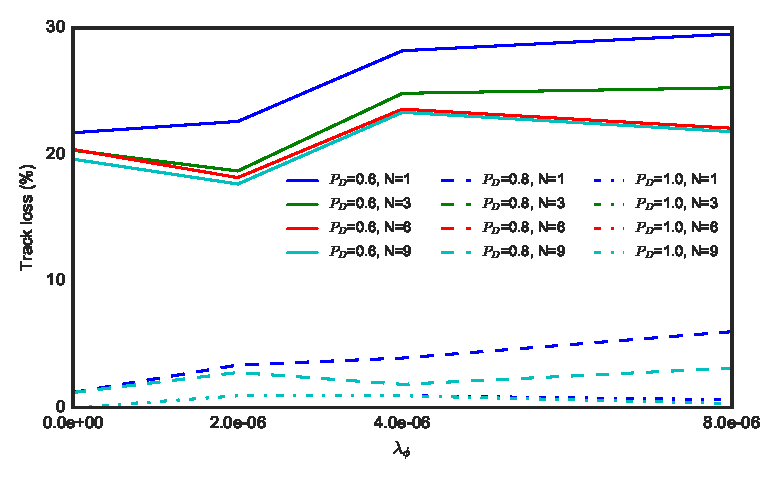
\includegraphics[height = .45\textheight]{Figures/plots/Scenario0_Tracking-TrackLoss.pdf}
\caption{Scenario 0 --- Track loss}\label{fig:scenario0_track_loss}
\end{figure}

\begin{figure}
\centering
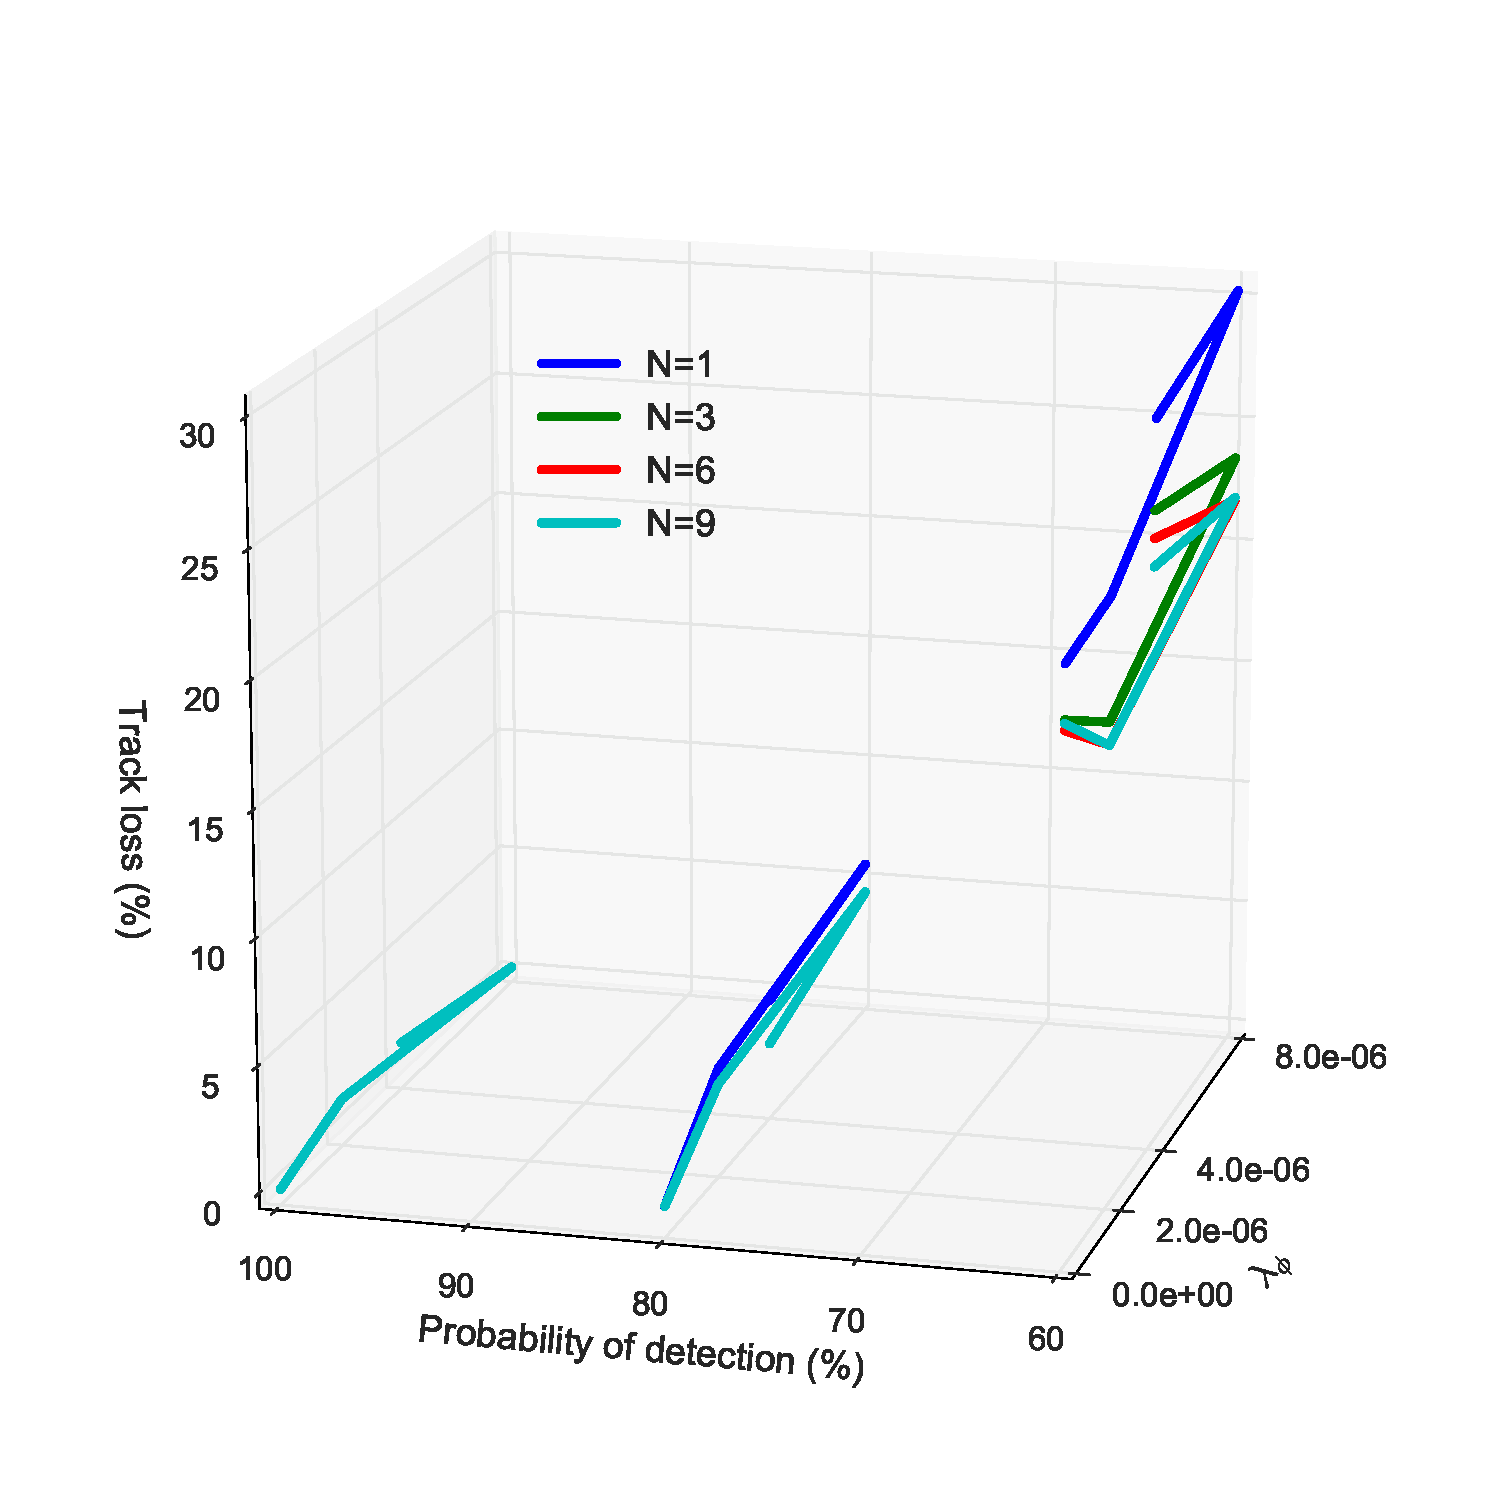
\includegraphics[height = .45\textheight]{Figures/plots/Scenario1_Tracking-TrackLoss.pdf}
\caption{Scenario 1 --- Track loss}\label{fig:scenario1_track_loss}

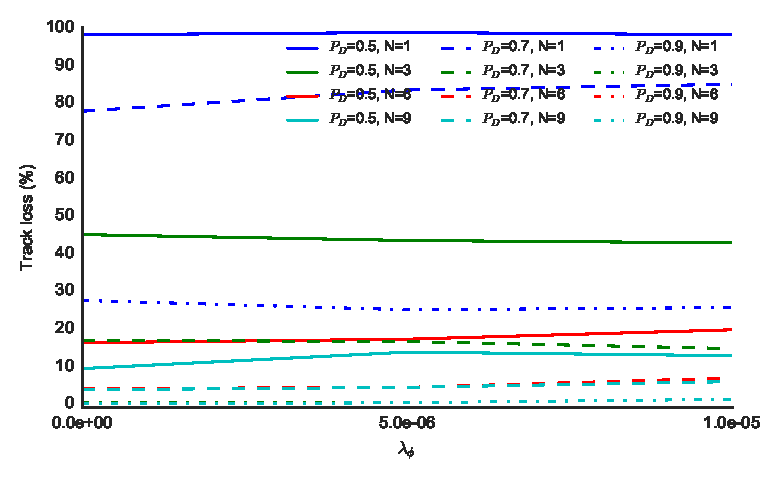
\includegraphics[height = .45\textheight]{Figures/plots/Scenario2_Tracking-TrackLoss.pdf}
\caption{Scenario 2 --- Track loss}\label{fig:scenario2_track_loss}
\end{figure}

\begin{figure}
\centering
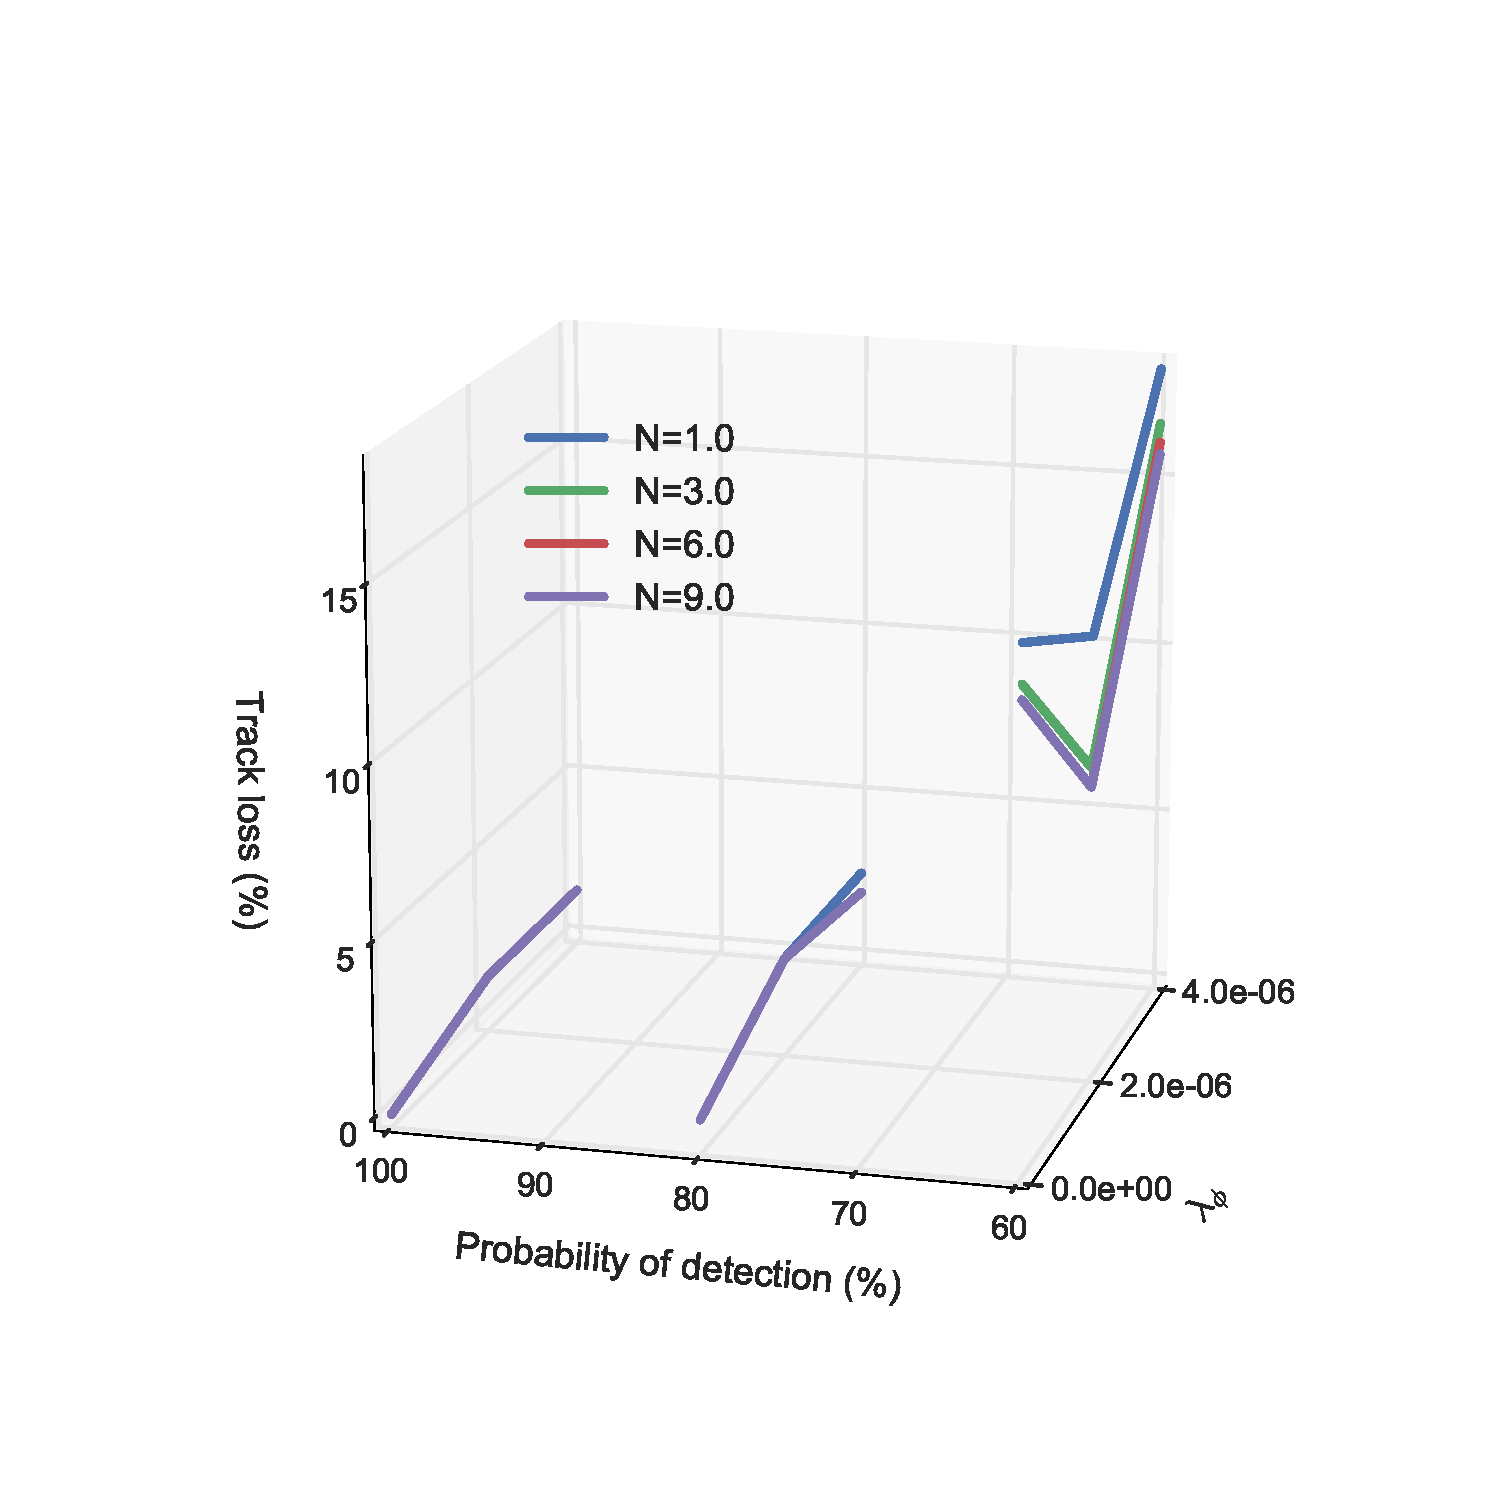
\includegraphics[height = .45\textheight]{Figures/plots/Scenario3_Tracking-TrackLoss.pdf}
\caption{Scenario 3 --- Track loss}\label{fig:scenario3_track_loss}

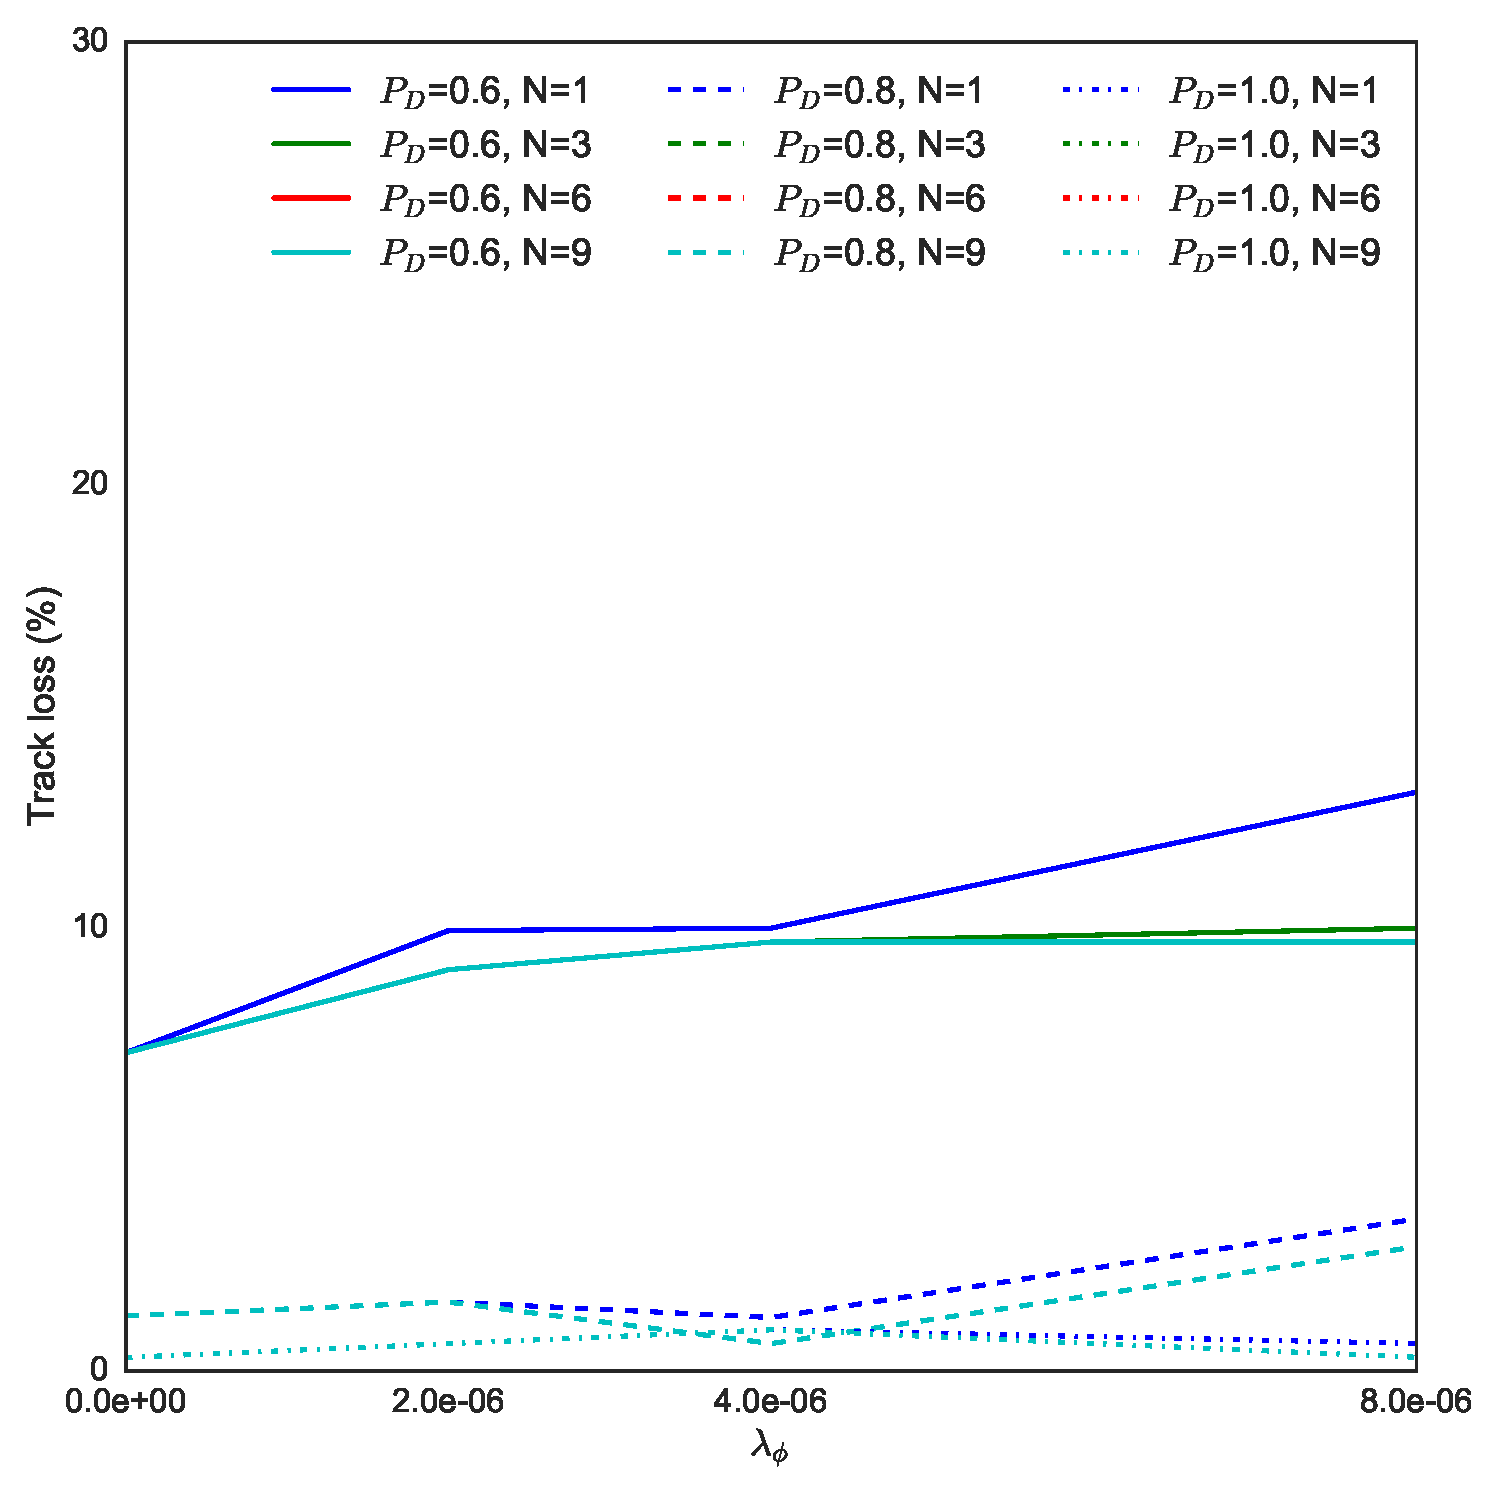
\includegraphics[height = .45\textheight]{Figures/plots/Scenario4_Tracking-TrackLoss.pdf}
\caption{Scenario 4 --- Track loss}\label{fig:scenario4_track_loss}
\end{figure}

}